\documentclass[12pt, letterpaper]{article}
\usepackage{bbold}
\usepackage{indentfirst}
\usepackage{amsmath, amssymb}
\usepackage[T1]{fontenc}
\usepackage[utf8]{inputenc}
\usepackage{physics}
\usepackage{tensor}
\usepackage{braket}
\usepackage{graphics}
\usepackage{grffile}
\graphicspath{ {/home/noor/Project/}}
\newcommand*{\1}{\hspace{1pt}}
\author{Noor E Mustafa Ferdous}

\title{}

\date{}

\begin{document}
    For 3-point connected Green funtion we get

    \begin{equation}
        \Gamma_{3}(G_{2})^{3} = - G_{3}
    \end{equation}

    Differentiating with respect to $\phi^{c}$

    \begin{align*}
        & \ \ \ \  \ \ \ \ \   \frac{\delta}{\delta \phi^{c}} \Gamma_{3}(G_{2})^{3} + \Gamma_{3}\frac{\delta (G_{2})^{3}}{\delta J}\frac{\delta J}{\delta \phi^{c}}  = \frac{\delta G_{3}}{\delta J}\frac{\delta J}{\delta \phi^{c}} \\ 
        & \implies \Gamma_{4}(G_{2})^{3} + 3 \Gamma_{3}(G_{2})^{2}G_{3}(G_{2})^{-1} = - G_{4}(G_{2})^{-1} \\ 
        & \implies \Gamma_{4} (G_{2})^{4} +3\Gamma_{3}(G_{2})^{2}G_{3}  = - G_{4} \\ 
        & \implies \Gamma_{4} (G_{2})^{4} -3\Gamma_{3}(G_{2})^{2}G_{2}\Gamma_{3}(G_{2})^{2}  = - G_{4} \tag*{[from eqn (1)]}
    \end{align*}

    Digramatically will be 

    \begin{figure}[h]
    \centering
    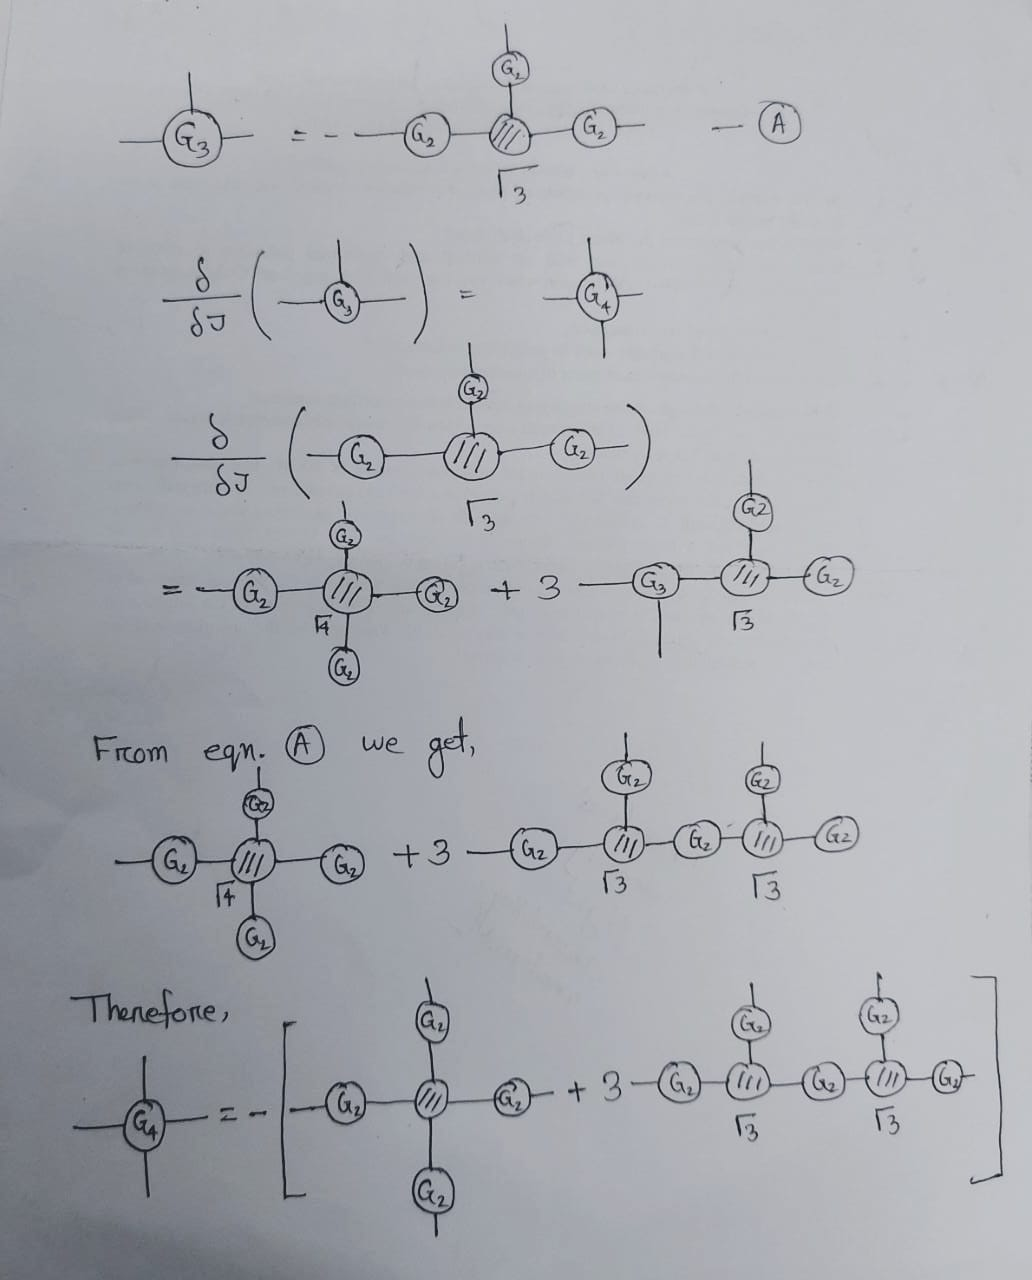
\includegraphics[scale=0.1]{spic}
    \end{figure}



    
\end{document}